\section{Omitted proof in  \cref{subsec: distance investment} 
 (investment)}\label{appendix: distance investment}


%-------------------
%--------------------------------------------
\begin{proof}[Proof of \cref{claim same behavior}]
    Consider any attributes $\features\notin\classifier_A\cap\classifier_B$. 
    We have shown that 
    if attributes $\features \in \setperp_A(\classifier_A,\classifier_B)$ or if attributes $\features \in \setperp_B(\classifier_A,\classifier_B)$, then the best response of any agent with such attributes is to take a one-step strategy.
    Hence it suffices to show for any attributes $\features \in \setonetwo_{\frac12}\cup\settwoone_{\frac12}$, there exists a one-step strategy  that is better than the best two-step strategy.

    \paragraph{Suppose  $\theta< 90^{\circ}$.}  The only  one-step strategy that could enable the agent to be selected is $\strategies(\features)=O$ (See \cref{fig:acute}).
    Notice that the cost of the one-step strategy is $\onecost(\features,O)=\eta \|\features - O\|_2$.
    Denote the distance between $\features$ and $O$ by $r= \|\features - O\|_2$.
    We distinguish three cases. 
    
    \begin{figure}
    \centering
  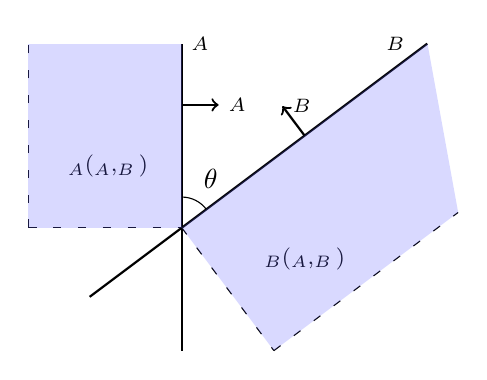
\begin{tikzpicture}[xscale=7.8,yscale=7.8]

\draw [domain=0.85:1.4, thick] plot (\x, {3/4*\x+1/4}) ;
\node [left] at (1.38, 1.3 ) {$\classifier_B$};%:\feature_2\geq \frac34 \feature_1 +\frac14
\draw [thick] (1,0.8) -- (1,1.3) ;
\node [right] at (1, 1.3) {$\classifier_A$};%: \feature_1 \geq 1$
\draw[black,thick,->] (1,1.2) -- (1.06,1.2)node[right]{$\weights_A$}; 
\draw[black,thick,->] (1.2,1.15) -- (1.2-0.06*0.6,1.15+0.06*0.8)node[right]{$\weights_B$}; 

% \node [left] at (1.33,1.25) {$+$};
% \node [right] at (1, 1.25) {$+$};
\draw (1,1)  ++(90-53.1:0.05) arc (90-53.1:90:0.05); \node[right] at(1.02,1.08){$\theta$};

\draw [domain=1+0.25*0.6:1.45, loosely dashed] plot (\x, {3/4*\x+1/4-5/16}); % 1/c = 1/4
\draw [loosely dashed] (1,1) -- (1+0.25*0.6,1-0.25*0.8);

\draw [loosely dashed] (1-0.25,1) -- (1-0.25,1.3);
\draw [loosely dashed] (1-0.25,1) -- (1,1);

\node[font=\tiny] at(0.88,1.1){\footnotesize$\setperp_A(\classifier_A,\classifier_B)$};
\node[font=\tiny] at(1.2,0.95){\footnotesize$\setperp_B(\classifier_A,\classifier_B)$};

\fill [blue!60,nearly transparent]  (0.75,1.3) -- (0.75,1) -- (1,1) -- (1,1.3)-- cycle;

\fill [blue!60,nearly transparent]  (1.4,5.2/4) --  (1,1) -- (1+0.25*0.6,1-0.25*0.8) --(1.45,5.35/4-5/16)-- cycle;
\end{tikzpicture}
\caption{$\theta<90^{\circ}$}
\label{fig:acute}
\end{figure}

    \paragraph{Case 1} Consider any attributes $\features$ that satisfy $\classifier_A$  but do not satisfy $\classifier_B$ (See \cref{fig: case 1}).
    Denote the angle between the vector $O\features$ and $-\weights_A$ by $\alpha$, where $\weight_A$ is the normal vector of $\classifier_A$ and $\alpha\in [0,90^{\circ}-\theta]$.
    In this case, $\features\in\settwoone_{\frac12}$, i.e., such attributes only have a profitable two-step strategy to first pass $\classifier_B$ then $\classifier_A$. 
    The best two-step strategy for $\features$ is $\strategies(\features)=(\features,\secondfeatures)$, where $\secondfeatures$ are the projection of $\features$ on the boundary line of $\classifier_A$.
    The cost of such a strategy is $\eta r \cos{\alpha}$.
    Hence the expected utility from the best two-step strategy is $\frac12-\eta r \cos{\alpha}$.
    Such attributes have a profitable two-step strategy, i.e., $\features\in \setonetwo_{\frac12}\cup\settwoone_{\frac12}$, if and only if $\frac12-\eta r \cos{\alpha}\geq 0$.
    
    It remains to show that 
    $$1-\eta r\geq \frac12-\eta r \cos{\alpha}, \text{ for all } r \text{ s.t. } \frac12-\eta r \cos{\alpha}\geq 0.$$
    It suffices to show 
    $$1\geq \frac{1- \cos{\alpha}}{\cos{\alpha}}\Leftrightarrow \cos{\alpha}\geq \frac12,$$ 
    which is true if $\theta\geq 30^{\circ}$.
    

\begin{figure}[t]
\centering
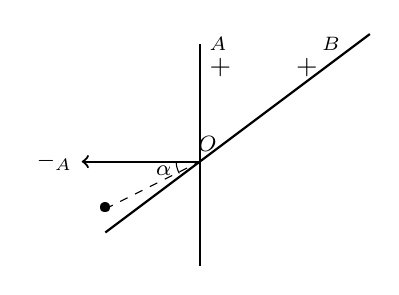
\begin{tikzpicture}[xscale=6,yscale=6]

\draw [domain=0.8:1.36, thick] plot (\x, {3/4*\x+1/4});
\node [left] at (1.32, 1.25 ) {$\classifier_B$};%:\feature_2\geq \frac34 \feature_1 +\frac14
\draw [thick] (1,0.78) -- (1,1.25);
\node [right] at (1, 1.25 ) {$\classifier_A$};%: \feature_1 \geq 1$
\node [left] at (1.27,1.2) {$+$};
\node [right] at (1, 1.2) {$+$};

\draw [->, thick]  (1,1)--(1-0.25,1);
\node [left] at (1-0.25, 1 ) {\footnotesize$-\weights_A$};

\node at (0.8, 0.9) {\textbullet};
\node [left] at (0.8, 0.9) {\footnotesize$\features$};
\draw[dashed](0.8, 0.9)--(1,1);
\draw (1,1)  ++({180}:0.05) arc (180:210:0.05); \node[left] at (0.96,0.98){\footnotesize$\alpha$};

\node [above] at (1.016, 1 ) {\footnotesize$O$};
\end{tikzpicture}
\caption{Case 1}
\label{fig: case 1}
\end{figure}


    \paragraph{Case 2} Consider any attributes $\features$ that satisfy $\classifier_B$  but do not satisfy $\classifier_A$ (See \cref{fig: case 2}).
    In this case, $\features\in\setonetwo_{\frac12}$, i.e., such attributes only have a profitable two-step strategy to first pass $\classifier_A$ then $\classifier_B$. 
Denote the angle between the vector $O\features$ and $-\weights_B$ by $\alpha$, where $\weight_B$ is the normal vector of $\classifier_B$ and $\alpha\in [0,90^{\circ}-\theta]$.
   The rest of the proof is analogous to case 1.

    \begin{figure}[t]
\centering
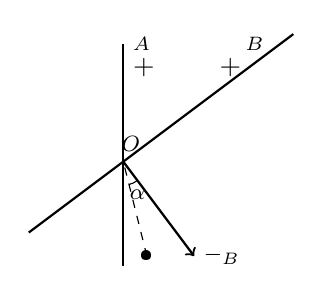
\begin{tikzpicture}[xscale=6,yscale=6]

\draw [domain=0.8:1.36, thick] plot (\x, {3/4*\x+1/4});
\node [left] at (1.32, 1.25 ) {$\classifier_B$};%:\feature_2\geq \frac34 \feature_1 +\frac14
\draw [thick] (1,0.78) -- (1,1.25);
\node [right] at (1, 1.25 ) {$\classifier_A$};%: \feature_1 \geq 1$
\node [left] at (1.27,1.2) {$+$};
\node [right] at (1, 1.2) {$+$};


 \draw [->,thick] (1,1) -- (1+0.25*0.6,1-0.25*0.8);
 \node [right] at (1+0.25*0.6,1-0.25*0.8) {\footnotesize$-\weights_B$};

\node at (1+0.05,1-0.2) {\textbullet};
\node [below] at (1+0.05,1-0.2){\footnotesize$\features$};
\draw[dashed](1+0.05,1-0.2)--(1,1);

\draw (1,1)  ++({270+atan(1/4)}:0.05) arc ({270+atan(1/4)}:{270+atan(3/4)}:0.05); 
\node[below] at (1.03,0.96){\footnotesize$\alpha$};

\node [above] at (1.016, 1 ) {\footnotesize$O$};
\end{tikzpicture}
\caption{Case 2}
\label{fig: case 2}
\end{figure}

    \paragraph{Case 3} Consider any attributes $\features$ that satisfy neither $\classifier_A$  nor $\classifier_B$.
    We first show that the best two-step strategy to first pass $\classifier_A$ and then $\classifier_B$ is less than the best one-step strategy.
    Similar argument can be used to show that the best two-step strategy to first pass $\classifier_B$ and then $\classifier_A$ is less than the best one-step strategy.
    
    Denote the symmetric attributes of $\features$ over the boundary line of $\classifier_A$ by $\tilde\features$ (See \cref{fig: case 3}).
    Then by symmetry, $r=\|\tilde\features - O\|_2$.
    Denote the projection point of $\tilde\features$ on the boundary line of $\classifier_B$ by $\secondfeatures$.
    Denote the (anti clockwise) angle between the vector $O\tilde\features$ and the boundary line of $\classifier_A$ by $\alpha$ (See \cref{fig: case 3}), where $\alpha\in [0,\theta]$.
    Then by symmetry, the best two-step strategy for $\features$ to first pass $\classifier_A$ and then $\classifier_B$ has the same cost as $\tilde\features$ moving to $\secondfeatures$, which is $\eta \|\tilde\features - O\|_2 \sin{(\theta+\alpha)}=\eta r \sin{(\theta+\alpha)}$.
 Hence the expected utility from the best two-step strategy to first pass $\classifier_A$ and then $\classifier_B$ is $\frac12-\eta r \sin{(\theta+\alpha)}$.
    Such attributes have a profitable two-step strategy to first pass $\classifier_A$ and then $\classifier_B$, i.e., $\features\in \setonetwo_{\frac12}\cup\settwoone_{\frac12}$, if and only if $\frac12-\eta r \sin{(\theta+\alpha)}\geq 0$.
    
    It remains to show that 
    $$1-\eta r\geq \frac12-\eta r \sin{(\theta+\alpha)}, \text{ for all } r \text{ s.t. } \frac12-\eta r \sin{(\theta+\alpha)}\geq 0.$$
    It suffices to show 
    $$1\geq \frac{1- \sin{(\theta+\alpha)}}{\sin{(\theta+\alpha)}}\Leftrightarrow \sin{(\theta+\alpha)}\geq \frac12,$$ 
    which is true if $\theta\geq 30^{\circ}$.
    Analogously, we can show that  if $\theta\geq 30^{\circ}$, then the best two-step strategy to first pass $\classifier_B$ and then $\classifier_A$ is less than the best one-step strategy.
    
    \begin{figure}[t]
\centering
\begin{tikzpicture}[xscale=8,yscale=8]

\draw [domain=0.76:1.36, thick] plot (\x, {3/4*\x+1/4});
\node [left] at (1.32, 1.25 ) {$\classifier_B$};%:\feature_2\geq \frac34 \feature_1 +\frac14
\draw [thick] (1,0.76) -- (1,1.25);
\node [right] at (1, 1.25 ) {$\classifier_A$};%: \feature_1 \geq 1$
\node [left] at (1.27,1.2) {$+$};
\node [right] at (1, 1.2) {$+$};


\draw [dotted] (1-0.1,1-0.2) -- (1+0.1,1-0.2);
\node at (1-0.1, 1-0.2 ) {\textbullet};
\node at (1+0.1, 1-0.2 ) {\textbullet};
\node [below] at (1-0.1, 1-0.2 ) {\footnotesize$\features$};
\draw [dotted]  (1+0.1,1-0.2) -- (1+0.1-5.45/24*0.6,1-0.2+5.45/24*0.8);
\node [below] at (1+0.1,1-0.2) {\footnotesize$\tilde\features$};
\node [left] at  (1+0.1-5.5/24*0.6,1-0.2+5.5/24*0.8) {\footnotesize$\secondfeatures$};
\node  at  (1+0.1-5.45/24*0.6,1-0.2+5.45/24*0.8) {\textbullet};

\draw [] (1,1) -- (1+0.1,1-0.2);
\draw (1,1)  ++({270}:0.05) arc (270:{300}:0.05); 
\node[below] at (1.04,0.96){\footnotesize$\alpha$};

\node [above] at (1.016, 1 ) {\footnotesize$O$};
\end{tikzpicture}
\caption{Case 3}
\label{fig: case 3}
\end{figure}

 \paragraph{Suppose  $\theta\geq  90^{\circ}$.}  By Theorem 3.7 in \citet{zigzag}, $\setonetwo_{\frac12}\cup\settwoone_{\frac12}$ is empty.
 Hence every agent prefers one-step strategy.
 



 \begin{figure}[h]  
\centering 
    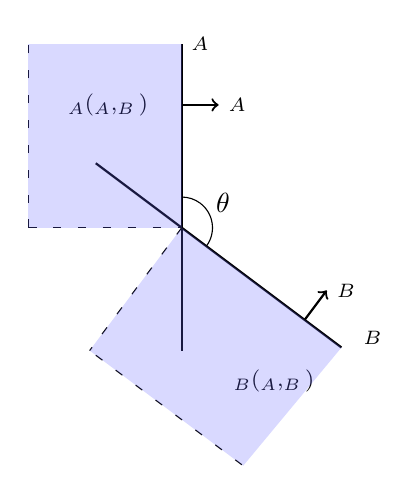
\begin{tikzpicture}[xscale=7.8,yscale=7.8]
% \draw [thick,->] (0.6,0.8) -- (1.5,0.8);
% \draw [thick, ->] (0.95,0.8) -- (0.95,1.32);
% \node [below] at (1.5,0.8) {$\feature_A$};
% \node [above] at (0.95,1.32) {$\feature_B$};

\draw [domain=0.86:1.26, thick] plot (\x, {-3/4*\x+7/4});
\node [right] at (1.28, 1-0.18 ) {$ \classifier_B$};%:\feature_2\geq \frac34 \feature_1 +\frac14
\draw [thick] (1,0.8) -- (1,1.3);
\node [right] at (1, 1.3) {$\classifier_A$};%: \feature_1 \geq 1$
\draw[black,thick,->] (1,1.2) -- (1.06,1.2)node[right]{$\weights_A$}; 
\draw[black,thick,->] (1.2,0.85) -- (1.2+0.06*0.6,0.85+0.06*0.8)node[right]{$\weights_B$}; 

\draw (1,1)  ++({-36.9}:0.05) arc (-36.9:90:0.05); \node[right] at (1.04,1.04){$\theta$};

% \draw[->] (1.25,1.15) --(1.25,1.25);
% \node[above]at (1.25,1.25){$\feature_b$};
% \draw[->] (1.25,1.15) -- (1.35, 1.15);
% \node[right]at (1.35,1.15){$\feature_a$};
% \node[left] at (1.25,1.15) {$O$};

\draw [domain=0.86:1.1, loosely dashed] plot (\x, {-3/4*\x+23/16});
\draw [loosely dashed] (1,1) -- (1-0.25*0.6,1-0.25*0.8);

\draw [loosely dashed] (1-0.25,1) -- (1-0.25,1.3);
\draw [loosely dashed] (1-0.25,1) -- (1,1);

\node[font=\tiny] at(0.88,1.2){\footnotesize$\setperp_A(\classifier_A,\classifier_B)$};
\node[font=\tiny] at(1.15,0.75){\footnotesize$\setperp_B(\classifier_A,\classifier_B)$};

\fill [blue!60,nearly transparent]  (0.75,1.3) -- (0.75,1) -- (1,1) -- (1,1.3)-- cycle;

\fill [blue!60,nearly transparent]  (1.26, -3/4*1.26+7/4) --  (1,1) -- (1-0.25*0.6,1-0.25*0.8) --(1.1,-3.3/4+23/16)-- cycle;

\end{tikzpicture}
\caption{$\theta\geq 90^{\circ}$}  
\label{fig:obtuse}
\end{figure}

\end{proof}

\begin{proof}[Proof of \cref{thm:optimal investment}]
    We show that the described simultaneous mechanism achieves the upper bound of the value of program \ref{max qualified}. 
    First notice that any qualified agent gets selected with zero cost under the described mechanism.
    Second, we show that the described mechanism accepts every unqualified agent who can improve to another qualified attributes with cost less than one.
    Consider an unqualified agent with attributes $\features\not\in\classifier_A \cap \classifier_B$. 
    Suppose there exists attributes $\features'$ such that (1)  $\features'$ satisfy both tests $\classifier_A$ and $\classifier_B$; and (2)  such an agent can move to $\features'$ with cost $c(\features, \features', \features') \leq 1$.
    Then this unqualified agent has an incentive  to improve his attributes to $\features'$ and get accepted.  
    However, if instead such attributes $\features'$ do not exist and for any attributes $\features''$ in $\classifier_A \cap \classifier_B$, the cost for this agent with attributes $\features$ to improve to $\features''$ is strictly larger than one, then this unqualified agent has no incentive to move to the qualified region $\classifier_A \cap \classifier_B$ in any mechanism.
    % While any unqualified agent with attributes in $\{\features : d(\features, \classifier_1\cap \classifier_2) > 1/\eta\}$ needs to pay a cost strictly greater than $1$ to reach qualified region $\classifier_1 \cap \classifier_2$.   
    Thus, the simultaneous mechanism that uses tests $\classifier_A$ and $\classifier_B$ accepts every agent who is either qualified or can improve their attributes to the qualified region with a cost less than one. 
    This is the upper bound of the value of program \ref{max qualified}.
    Hence the described simultaneous mechanism is optimal.
\end{proof}